\documentclass[11pt]{article}
\usepackage[margin=1in]{geometry}
\usepackage{amsmath,amssymb}
\usepackage{siunitx}
\usepackage{graphicx}
\usepackage[hidelinks]{hyperref}
\usepackage{enumitem}
\graphicspath{{figures/}}

\title{\texttt{PTCryspMC.jl} --- The application\\[2pt]
\large Phantom-based and proton-beam-based PET simulation}
\author{}
\date{}

\begin{document}
\maketitle
\begin{abstract}
\noindent
\texttt{PTCryspMC.jl} produces, for a given PET scanner, the list of coincidences it would record.
The detector response is computed by the engine described in the companion document
\texttt{PTCryspMC\_phys}; this document describes how that engine is driven. The simulator runs in
two modes that differ only in where the annihilations come from: a \emph{phantom-based} mode, in
which a geometric phantom is filled with a uniform source, and a \emph{proton-beam-based} mode, in
which the source is the positron activity a proton dose leaves. The phantom mode is complete and is
described in full; the proton-beam mode, the eventual target, is outlined.
\end{abstract}

\tableofcontents

\section{Introduction}

The purpose of the simulator is to generate, for each candidate scanner, the list-mode file of lines
of response (LORs) that a measurement would yield. That list is the input to a separate analysis
that recovers the proton range; the analysis is independent of the simulation and is described
elsewhere.

The engine --- the physics, geometry, transport, and detector model --- is the same in both modes.
What changes between them is the \emph{source}: the spatial distribution of the annihilation points
and the rate at which they occur in time.

\begin{description}[style=nextline,leftmargin=1.5em]
\item[Phantom-based mode.] The annihilations fill a geometric phantom --- a sphere or cylinder of
water --- with a uniform activity. The source is controlled and has an analytic ground truth, which
makes this mode the one in which the engine and the detector model are validated, and a study tool
in its own right.
\item[Proton-beam-based mode.] The annihilations are drawn from a \emph{scenario}: the positron
activity a proton field leaves, computed upstream and frozen. This is the measurement the simulator
ultimately serves.
\end{description}

Both modes produce the same deliverable: a list-mode file in which every LOR carries its two hit
positions, energies and times, and a flag marking it as a \emph{true}, \emph{scatter}, or
\emph{random} coincidence.

\section{Phantom-based mode}
\label{sec:phantom}

\subsection{The phantom source}

The source is a geometric solid placed at the centre of the ring: a water sphere or cylinder.
Annihilation points are drawn uniformly by volume inside it, and each point emits a back-to-back
pair as described by the engine. The same solid is also the attenuator --- it both emits the photons
and scatters them --- so a water phantom produces realistic patient scatter, while a vacuum phantom
of the same shape gives the non-attenuated reference against which the attenuation is measured. The
number of annihilations is set directly in the run configuration.

\subsection{The run configuration}

A run is specified by a single TOML file with sections for the geometry, the source, the transport,
the detector, and the timing. The file name is the run \emph{tag}, which names the output directory
and is stamped into every output, so a run carries its own provenance. Naming the crystal in the
transport section pulls all of that crystal's properties (cross sections, light yield, scintillation
decay, resolution, efficiency) from the materials database.

\subsection{The activity model}

The annihilations are spread in time by an activity model. For a single isotope decaying with
constant $\lambda = \ln 2 / T_{1/2}$ over an acquisition window $[t_0, t_1]$, the activity is
$A(t) = A_0\, e^{-\lambda (t-t_0)}$, so each event's annihilation time is drawn from a truncated
exponential on that window. Figure~\ref{fig:activity} shows the curve for the default isotope,
$^{15}$O ($T_{1/2} = \SI{2.04}{min}$): the activity is front-loaded, densest at the start of the
acquisition. The time of each event is computed deterministically from its event number, so it is
the same however the events were distributed across threads, and identical in every pass that reads
it. This per-event time is what the randoms pass needs.

\begin{figure}[t]
  \centering
  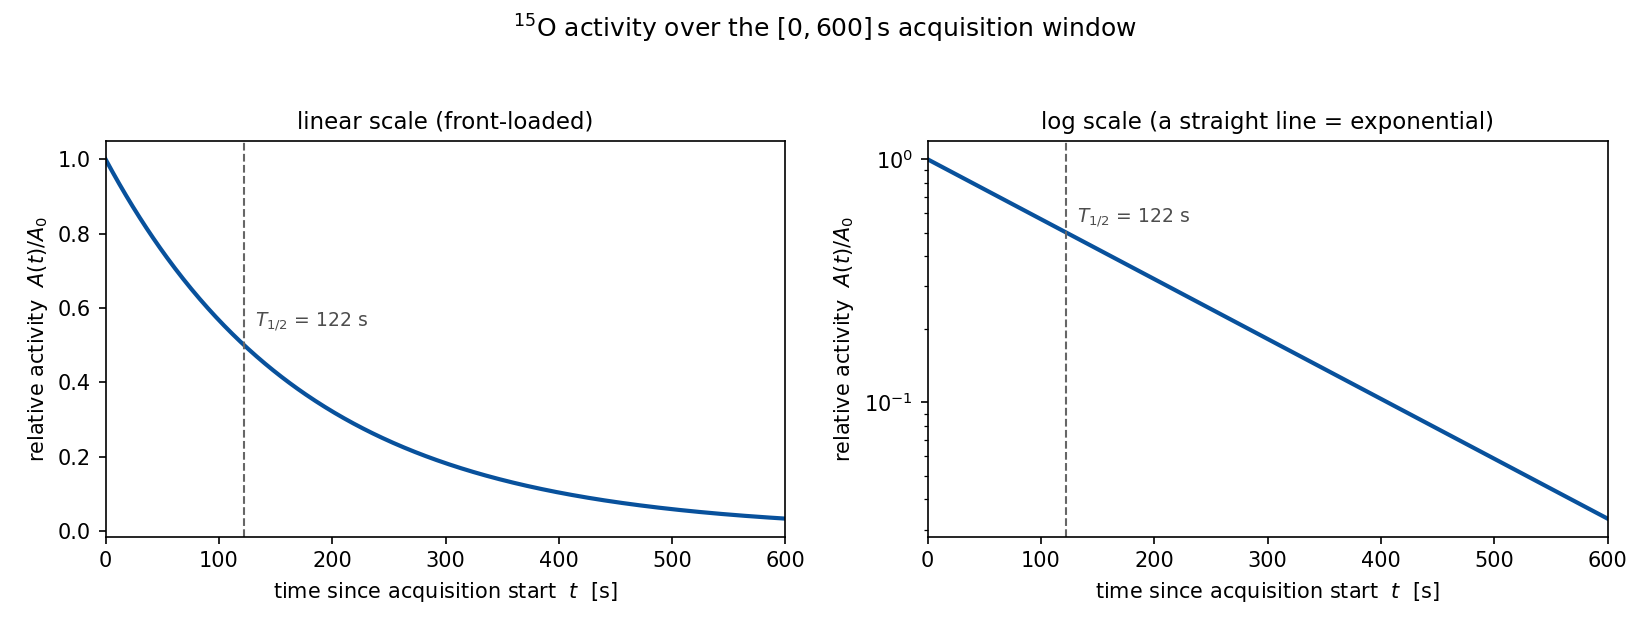
\includegraphics[width=\textwidth]{activity}
  \caption{The source activity over the acquisition window for $^{15}$O. The annihilation times
  follow the truncated exponential $A(t)\propto e^{-\lambda(t-t_0)}$ --- front-loaded, which is the
  origin of the randoms' front-loading.}
  \label{fig:activity}
\end{figure}

\subsection{The production chain}

The measurement is built in stages, each a streaming pass that scales to the large event counts a
run contains (Table~\ref{tab:chain}).

\paragraph{Singles.} \texttt{simulate\_source\_mt} draws the annihilations and transports their
photons, writing one row per detected photon: its first-interaction point and block, its summed
energy, and its time $t_{\mathrm{rel}}$ relative to the decay --- the time of flight plus the
scintillation jitter --- stamped once, here, so that every later stage reuses the same per-photon
time. The pass is multi-threaded over contiguous blocks of events.

\paragraph{True coincidences.} \texttt{build\_true\_coincidences\_from\_singles} pairs the two
photons of each annihilation that both reached the ring contained in one block. Each pair becomes a
LOR carrying the two timestamps $t_1, t_2$ and the residual $\mathrm{d}t = (t_1 - t_2) -
\mathrm{TOF_{diff}}$, in which the geometric time-of-flight difference is removed so that
$\mathrm{d}t$ measures the timing resolution alone. These are the true and scatter coincidences.

\paragraph{The coincidence window.} Two photons are a coincidence when their arrival times fall
within a window $\tau$. The window is read off the measured distribution of
$\Delta T = |t_1 - t_2|$ (Fig.~\ref{fig:dt}): a few-nanosecond window already keeps almost every
genuine pair. The chosen $\tau = \SI{3}{ns}$ keeps about $99\%$ of the coincidences. Because
$\Delta T$ is set mainly by the spread in time of flight across the ring --- geometry, not the
crystal --- the same window serves both CsI and BGO.

\begin{figure}[t]
  \centering
  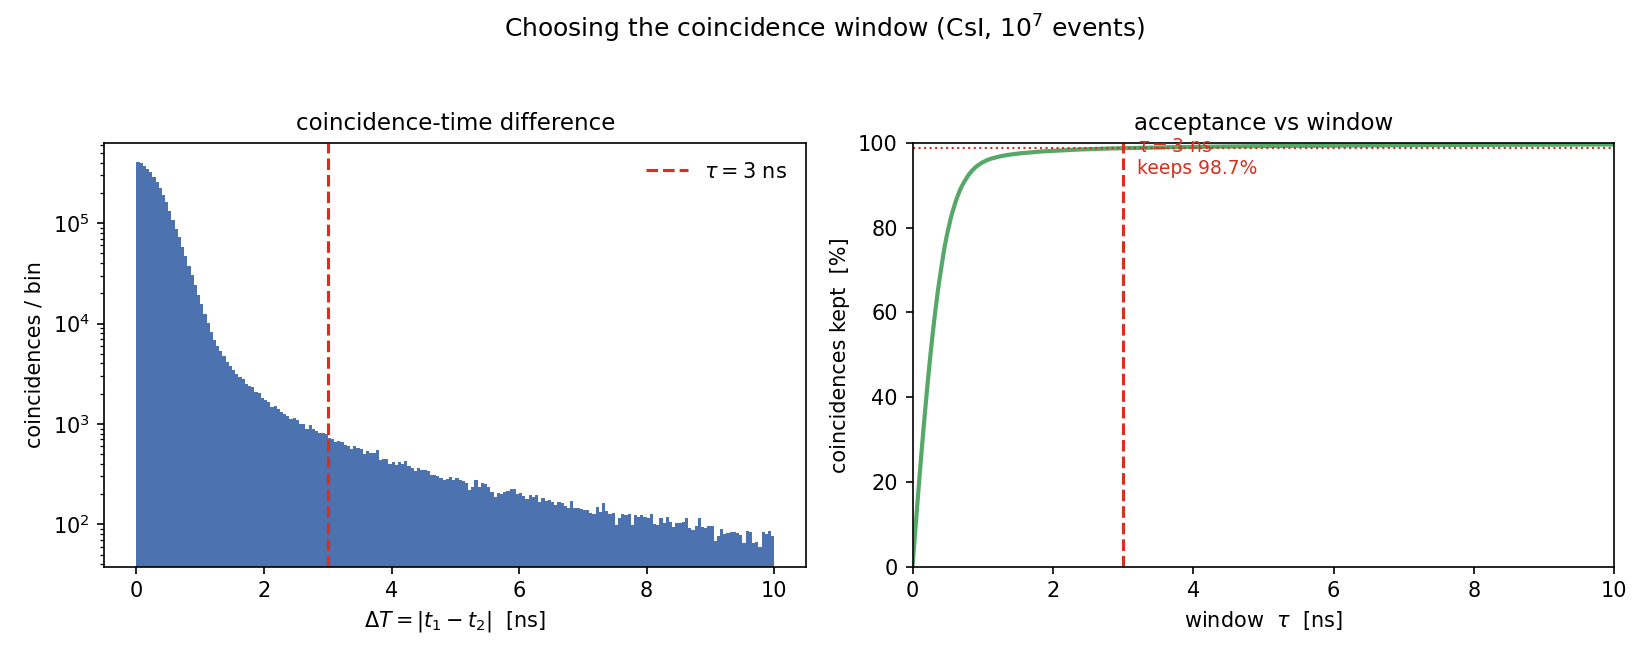
\includegraphics[width=\textwidth]{dt}
  \caption{Choosing the coincidence window. Left, the distribution of the coincidence-time
  difference $\Delta T = |t_1 - t_2|$. Right, the fraction of coincidences kept as the window $\tau$
  is widened. The window $\tau = \SI{3}{ns}$ (dashed) keeps about $99\%$ of the pairs.}
  \label{fig:dt}
\end{figure}

\paragraph{Randoms.} \texttt{build\_randoms\_from\_singles} forms the accidental background. It pairs
singles from \emph{different} annihilations whose absolute arrival times --- the decay time plus
$t_{\mathrm{rel}}$ --- fall within $\tau$. Because two unrelated decays must coincide to within a few
nanoseconds, randoms are rare and front-loaded: their rate is approximately $2\tau S^2$ in the
singles rate $S$, so it follows the square of the activity and fades faster than the true rate.

\paragraph{Reconstructed coincidences.} \texttt{reco\_lors} merges the trues and the randoms into the
detector-level measurement. It applies the detector response (position and energy smearing), the
energy selection, and the coincidence-window cut $|t_1 - t_2| \le \tau$, and flags every surviving
LOR as true, scatter, or random. The energy selection is a lower cut on the smeared energy
(Fig.~\ref{fig:spectrum}). Detector studies keep this cut low (\SI{300}{keV}) so the Compton
shoulder remains visible in the spectrum; the reconstruction raises it to the photopeak region
(\SI{450}{keV}), which selects full-energy events, suppresses scatter, and shrinks the file.

\begin{figure}[t]
  \centering
  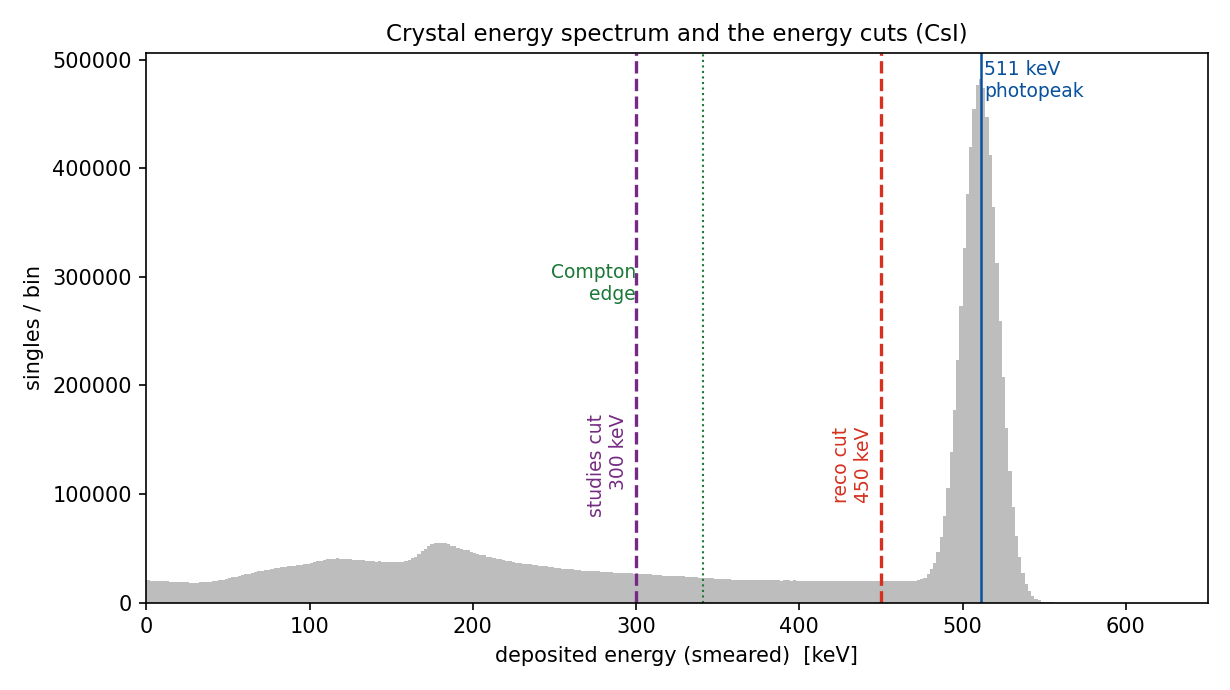
\includegraphics[width=0.78\textwidth]{spectrum}
  \caption{The crystal energy spectrum (CsI, smeared by the $5\%$ resolution): the full-absorption
  photopeak at \SI{511}{keV} above the Compton continuum, with its edge near \SI{341}{keV}. The two
  lower energy cuts are marked --- the low studies cut keeps the shoulder, the higher reconstruction
  cut selects the photopeak.}
  \label{fig:spectrum}
\end{figure}

\begin{table}[h]
  \centering
  \begin{tabular}{lll}
    \hline
    stage & script & output \\
    \hline
    transport      & \texttt{simulate\_source\_mt}                  & \texttt{singles.h5} \\
    true pairing   & \texttt{build\_true\_coincidences\_from\_singles} & \texttt{lors\_truth.h5} \\
    randoms        & \texttt{build\_randoms\_from\_singles}         & \texttt{randoms.h5} \\
    reconstruction & \texttt{reco\_lors}                            & \texttt{lors\_det.h5} \\
    \hline
  \end{tabular}
  \caption{The production chain. Each stage is a streaming pass; the singles list, written once, is
  read by both the true-coincidence and the randoms stages.}
  \label{tab:chain}
\end{table}

\subsection{The list-mode output}

The deliverable is \texttt{lors\_det.h5}: one record per coincidence, carrying the two hit positions,
the two energies, the two times, the timing residual, and the truth flag. The flag separates the
three populations a real scanner mixes --- the true coincidences that carry range information, the
scatter coincidences that misposition it, and the random coincidences that add a flat background ---
so the downstream analysis can study each on its own.

\subsection{Validation}

Phantom mode is where the engine is checked against known answers. Transporting \SI{511}{keV} photons
through the water phantom reproduces Beer--Lambert attenuation (the unscattered fraction
$0.215$ against the analytic $0.216$). The random rate matches the analytic $2\tau S^2$ to within
the statistical uncertainty. The timing residual $\mathrm{d}t$ matches the single-photon jitter
predicted from the crystal's light yield and decay. And the full chain runs the order of $10^{8}$
annihilations in a few minutes. Across crystals, the denser BGO contains more full-energy events
than CsI (a higher acceptance after the photopeak cut), while its lower light yield gives it a
coarser timing resolution --- both as the physics predicts.

\section{Proton-beam-based mode}
\label{sec:proton}

This is the mode the simulator ultimately serves. It is outlined here; the implementation follows.

\subsection{The idea}

A proton beam delivering a therapeutic dose fragments nuclei along its path, leaving short-lived
$\beta^+$ emitters --- $^{15}$O, $^{11}$C, and others. Their positrons annihilate nearby, so the
dose leaves a positron-activity image whose distal edge tracks the proton range. Imaging that
activity with PET, and comparing the measured range to the plan, is the verification this simulator
supports.

The upstream code \texttt{ptcryspg4} transports the protons and the positrons and freezes a
\emph{scenario}: the set of annihilation points --- the spatial source, with the positron range
already contained in each point --- together with, for each isotope, the number of decays measured
(the budget) for a given dose and acquisition timing. The scenario is the bridge between the beam
and this simulator.

\subsection{What changes from phantom mode}

Only the front of the chain changes. The source becomes the scenario: annihilation points are drawn
from the scenario's emitters, per isotope and to the measured budget, in place of the uniform draw
in a geometric solid. The activity model becomes the per-isotope mixture the scenario specifies, in
place of the single toy isotope. Everything downstream --- the transport, the singles list, the true
and random coincidences, the reconstruction, and the list-mode output --- is unchanged. The
machinery validated in phantom mode runs without modification on the scenario source.

\subsection{Status}

The scenario reader and the per-isotope injection are the remaining piece. The phantom mode provides
the validated engine and chain they will feed; this section will be expanded as the scenario format
is fixed.

\section*{Reference material}
\addcontentsline{toc}{section}{Reference material}
The detector model and the geometry are described in \texttt{PTCryspMC\_phys}. The CRYSP detector
numbers follow Soleti \textit{et al.} (2024); the upstream scenario method is documented with
\texttt{ptcryspg4}.

\end{document}
